\documentclass[epsfig,a4paper,12pt,titlepage,twoside,openany]{book}

% Main packages used
\usepackage{epsfig}
\usepackage{plain}
\usepackage[paperheight=29.7cm,paperwidth=21cm,outer=1.5cm,inner=2.5cm,top=2cm,bottom=2cm]{geometry}
\usepackage{titlesec}
\usepackage[english]{babel}
\usepackage[utf8x]{inputenc}
\usepackage[colorlinks=true, allcolors=blue]{hyperref}
\usepackage{enumitem}
\usepackage{float}
\usepackage{titlesec}
\newcommand{\retrievalDate}{25th of October, 2017}
\setlength{\parindent}{0pt}
\addto\extrasenglish{%
  \renewcommand{\chapterautorefname}{Chapter}%
}

% https://github.com/Angtrim/alloy-latex-highlighting
\usepackage[dvipsnames]{xcolor}
\usepackage{listings}
\usepackage{./alloy/alloy-style}
\usepackage[figuresright]{rotating}

\begin{document}
	\pagenumbering{gobble}
	\pagestyle{plain}

\thispagestyle{empty}

\begin{center}
	\begin{figure}[h!]
    	\centerline{
\psfig{file=images/logo_polimi.png,width=0.6\textwidth}}
  	\end{figure}

	\vspace{2 cm} 
  	\Large\textsc{Travlendar+ $\vert$ Software Engineering II Project\\} 
  	\vspace{1 cm} 
  	\Huge\textsc{Design Document\\}

  	\vspace{2 cm}
  	\begin{tabular*}{\textwidth}{ c @{\extracolsep{\fill}} c @{\extracolsep{\fill}}}
  		\Large{\it{Authors}} & \Large{\it{Professor}}\\
  		\Large{Antonio Frighetto} & \Large{Elisabetta Di Nitto}\\
  		\Large{Leonardo Givoli}\\
  		\Large{Hichame Yessou}\\
	\end{tabular*}

  	\vspace{5 cm} 

  	\Large{Academic year 2017/2018}
\end{center}


	\clearpage

	\tableofcontents
	\mainmatter
    
	% Sections
	\begingroup
		\chapter{Introduction}
\label{cha:intro}

\section{Purpose}
\label{sec:purpose}
Here is a brief description of what this document, namely \textit{Requirements Analysis and Specification Document} (RASD), aims to cover, and an initial context of the problem and its goals are illustrated thereafter. \\\\
The ultimate goal of RASD is to give an understanding of the customer requirements by describing the system itself, its functional and non-functional requirements, its components and constraints, and the relationship with the external world so that such system can be modeled with regard to the customers' needs. It is mainly addressed to project managers, systems analysts, developers, testers, and can be useful to final users as well. Being legally binding, it may be used in a contractual requirement.\\\\
Travlendar+ is an intelligent calendar-based time-aware cross-platform application, whose goal is to simplify and augment the way the final user is used to handling its own events and appointments. Users will feel free to create as many meetings as they may need, and it will be up to the application to manage them by arranging such appointments according to the travel time and the his or her position so as to ensure that he or she is not going to ever be late. This implies that the application must recognize what kind of transport mean is best to reach specific locations, be it public or private, shared or not. Should it be a public mobility option and tickets purchase be available for that city, then the user may be able to buy them directly within the application. Likewise, should a bike sharing system exist nearby, then it would be surely prompted to the user - provided that he would arrive to the destination early enough. In any case, while the application will possibly suggest the best transport mean (or a combination) of them to the user, he or she can eventually choose the one that suits him or her best, according to his or her needs or wishes.
Besides the aforementioned features, the application is provided with an additional module:
\begin{description}
\item[Lunchtime event:] it allows the user to insert an event for lunch at whatever time he or she wants, as long as it fall into a range of hours, and events will be rearranged accordingly.
\end{description}
Let us now point out the main goals in more detail. From here on, the term \textit{users} clearly refers to registered users.
\begin{itemize}
\item {[G0]} Allow unregistered user to sign up to access to the application.
\item {[G1]} Allow registered users to log in and access the application and start viewing their appointments.
\item {[G2]} Allow users to create meetings by entering a title, date and time, and the location of the event, and optionally, a description, and the type of event.
\item {[G3]} Allow users to select a maximum time interval for a certain event.
\item {[G4]} Allow users to modify and delete newly created events.
\item {[G5]} Give users a friendly overview of the day's events and the scheduled time to reach a location alongside the travel mean to be used.
\item {[G6]} Show users public and private transportations (or a combination of them) available for a specific trip.
\begin{itemize}
\item {[G6.1]} Provided results must have been undergone to a selection which may depend on unavailability of specific transport for a particular day or, for instance, climate conditions.
\item {[G6.2]} Prevent users from suggesting transports which are, say, out of scope (if two locations are pretty near, then they can be reached on foot, or after a certain hour a transport may be suspended). 
\item {[G6.3]} Allow users to deactivate specific settings, such as driving (in case of inability to drive), tolls (in case of willingness to free-only routes), or enable settings that may use only sustainable transports.
\item {[G6.4]} Allow users to benefit from results found, like sharing systems or own vehicles, if provided by the user.
\end{itemize}
\item {[G7]} Give users the chance to customize the travel mean by themselves, after suggesting the best mobility options that can be taken.
\item {[G8]} If enabled, alert users whether a specific locations is not reachable in the expected time.
\item {[G9]} If enabled, alert users whether a specific meeting is taking longer than expected.
\item {[G10]} Allow users to buy in-app tickets for public transportation or book a taxi.
\item {[G11]} Allow users to insert events with flexible time occupation (lunch). 
\end{itemize}

\section{Scope}
\label{sec:scope}
There exist phenomena that occur in reality but cannot be observable by the application, and phenomena which are controlled by the system and are unreachable from the outside. The connection between the world and the machine is made possible by the shared phenomena. \\\\
Here we include an analysis of the world and of the shared phenomena.
\paragraph{World phenomena}
\begin{itemize}
\item User is physically unable to open and use the application.
\item User's appointment takes longer than expected.
\item User accidentally messes up or a glitch takes place. 
\item User's own vehicles run out of gasoline.
\item A shared bicycle damages.
\item Public transport goes out of work.
\item Weather unexpectedly changes.
\item Location becomes unreachable.
\item Tickets are sold out.
\end{itemize}
\paragraph{Shared phenomena}
\begin{itemize}
\item User logs into the system.
\item User's appointment creation.
\item Warn if appointment is getting closer.
\item User buys a bus (or train) ticket or books a taxi.
\item Following an accident, appointments are rearranged.
\item Public transports changes are reported in real time.
\item Potential weather changing is reported in time.
\end{itemize}
\section{Definitions}
\label{sec:defs}
\begin{description}
\item[RASD:] Requirements Analysis and Specification Document (this document).
\item[System:] the whole software system to be developed, comprehensive of all its parts and modules. System and application are often used interchangeably. 
\item[User:] any user that downloads the application and, after registering, starts using it.
\item[Calendar-based:] what it shows up is a timeline for the current day or a calendar grid. 
\item[Time-aware:] it automatically recognizes when specific events occur, prevent events from overlapping among each other.
\item[Cross-platform:] multiple computing platforms are supported.
\item[API:] Application Programming Interface.
\end{description}

\section{References}
\label{sec:refer}

This document follows the IEEE 29148:2011\cite{ieee-29148} for the requirements engineering for systems and software products and IEEE 830-1998\cite{ieee-830} for the recommended practice for software requirements specifications.

It is based on the specifications document of the RASD assignment\cite{assignment}.

\section{Overview}
\label{sec:overview}

This document is structured as follows:
\begin{description}
\item[\autoref{cha:intro}: Introduction.] It provides a general description of the system purpose and scope, along with some information about this document.
\item[\autoref{cha:desc}: Overall description.] It provides the underlying perspective over the principal system features, constraints and those factors which affects the product.
\item[\autoref{cha:requirements}: Specific requirements.] It specifies thoroughly functional and nonfunctional requirements.
\item[\autoref{cha:modeling}: UML modeling.] It provides the use-case diagram, use cases descriptions, sequential diagrams, and other ones.
\end{description}
We conclude with an \textbf{Appendix}, which consists of the Alloy model, software and tools used, and hours of work per each team member and a \textbf{Bibliography}.

		\newpage
		\chapter{Overall Description}
\label{cha:desc}

\section{Product perspective}
\label{sec:productperspective}
The application will be available through web and mobile devices, keeping the same look and elements along the various implementations.
The user experience through the application should be easy and natural.
\\The application developed allow the time slotting ahead the upcoming events so that the user can have a full view of the day with a prediction of the travel time between the appointments if they are in different locations.
The event can regard working or personal aspects, and in any case, the application will notify or suggest a different mean of transport based on the weather conditions or strikes of the public transport.

\section{Product functions}
\label{sec:productfunctions}
The application allows you to schedule events, choose which mean of transport and get warned in case of overlapping events
On top of the time allocation, there will be a cost estimation provided when possible. 
This will allow the user to filter the possible mean of transport based on carbon footprint emission, price impact and time.

A User can:
\begin{itemize}
\item Create an event:
\begin{itemize}
\item Modify an event
\item Invite other users to their events
\end{itemize}
\item Receive help to reach the location of the next event
\begin{itemize}
\item Buying tickets for a mean of transport that require tickets
\item Providing navigation for reaching the spot 
\end{itemize}
\end{itemize}
\begin{itemize}
\item Get notified
\begin{itemize}
\item Upcoming events
\item Free space
\end{itemize}
\end{itemize}


\begin{figure}[H]
  \centerline{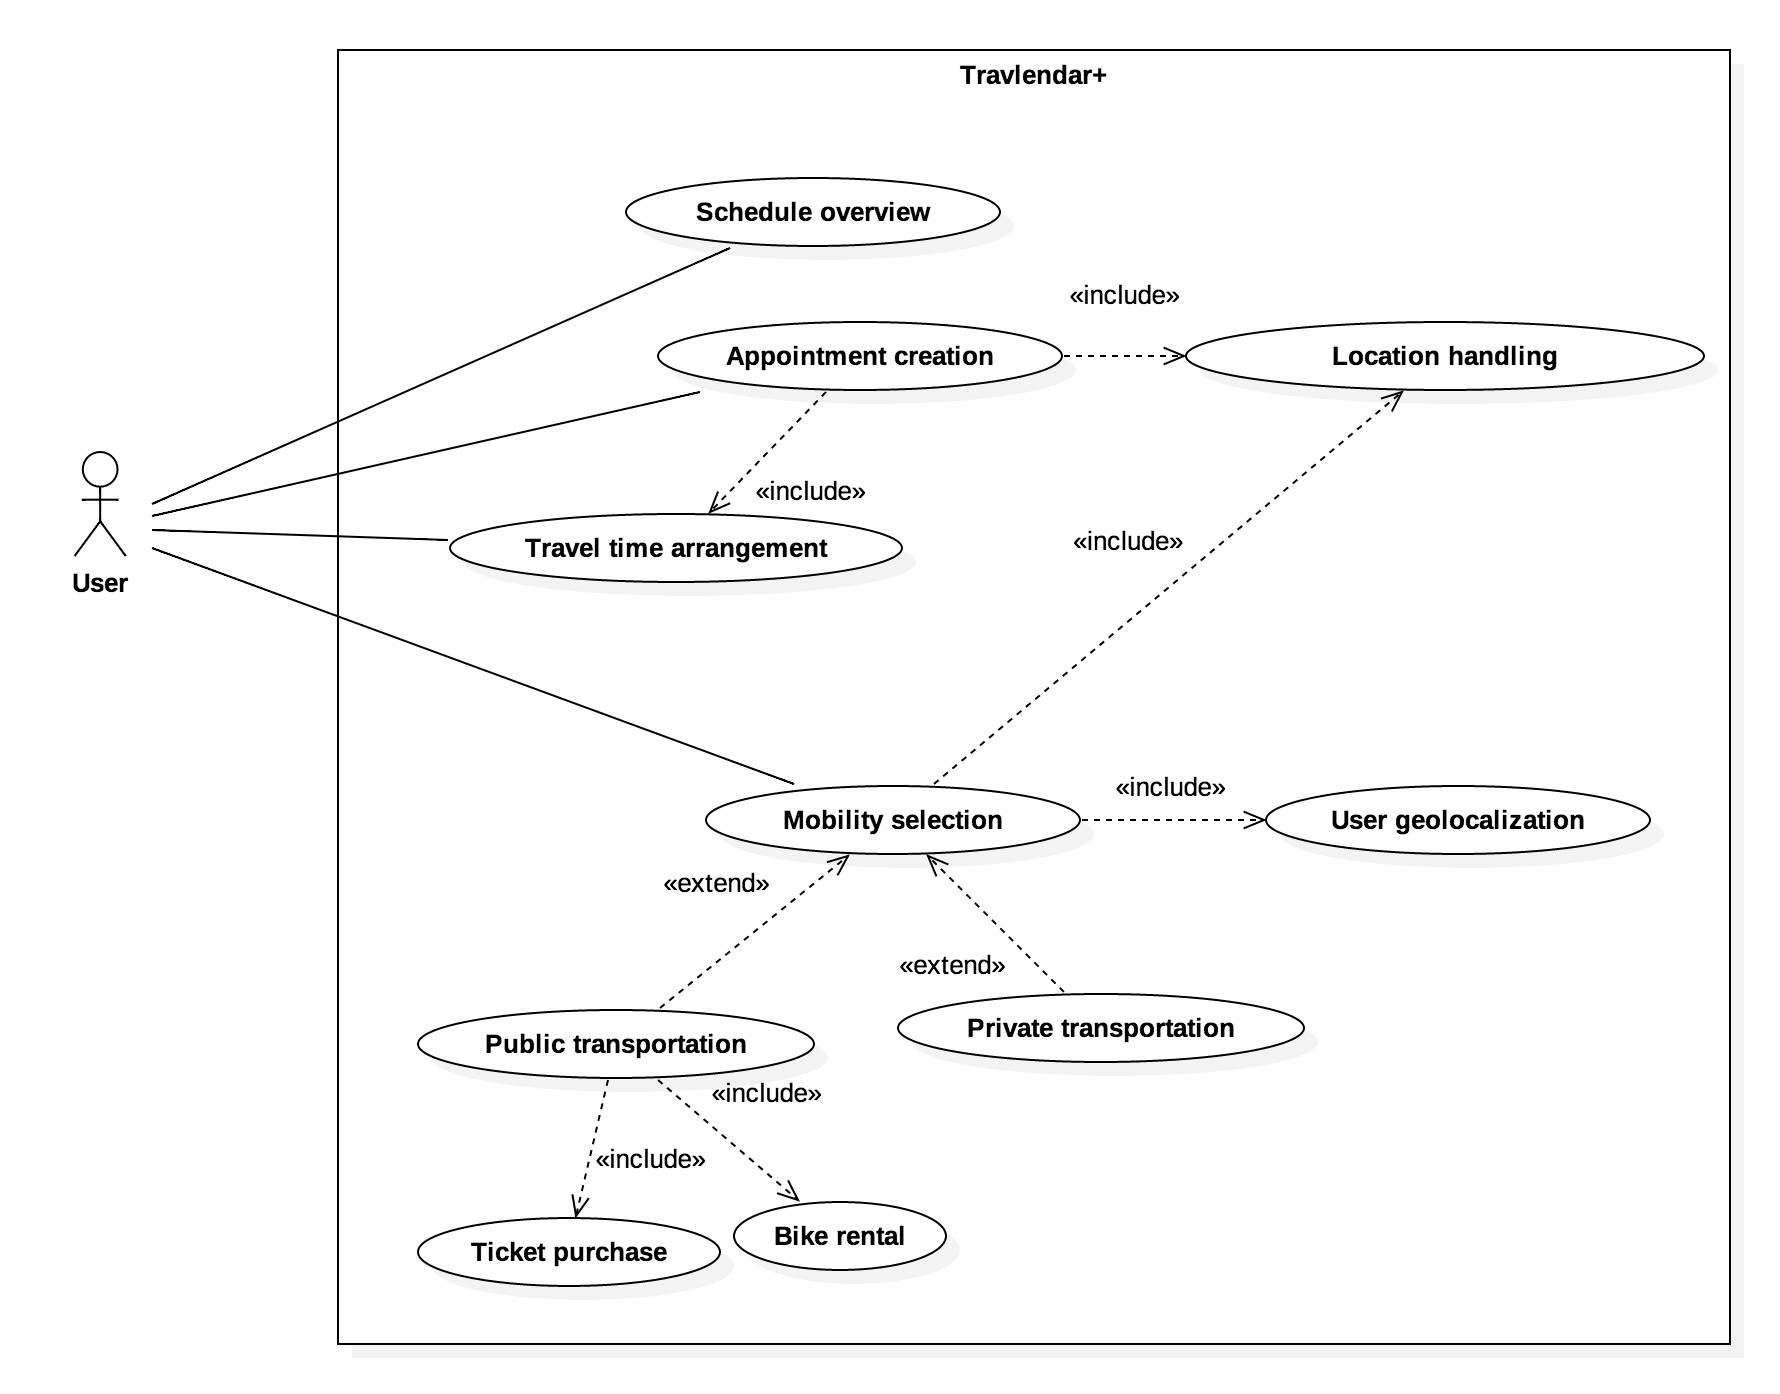
\psfig{file=diagrams/UseCaseDiagram.png,width=\textwidth} }
  \caption{Comprehensive use case diagram.}   
\end{figure}

\begin{figure}[H]
 \centerline{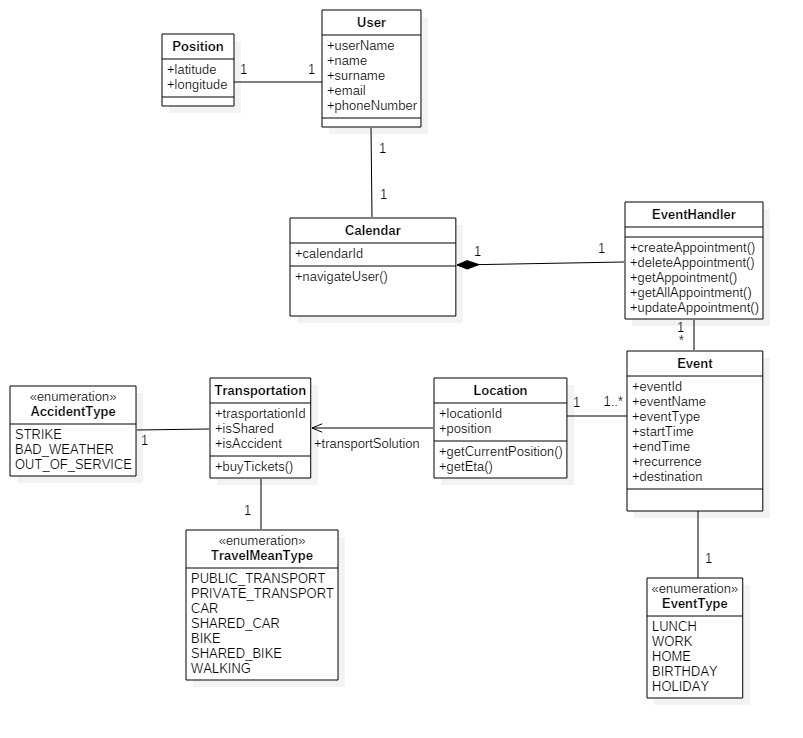
\psfig{file=diagrams/ClassDiagram.png,width=\textwidth} }
 \caption{Comprehensive class diagram.}  
\end{figure}

\section{User characteristics}
\label{sec:usercharacteristics}
\begin{description}
\item There is one type of user, which can be interfaced with other users in case of shared meetings.
\item Instead, the users that receive the invite will have read-only permissions.
\end{description}



\section{Assumptions, dependencies and constraints}
\label{sec:assumpdepenconst}

\paragraph{Text assumptions}
\begin{itemize}
\item The user will be able to schedule only future events, with the option to recur on a daily, weekly or monthly basis.
\item The working events can only be scheduled within the working hours, reserving at least 30 minutes for the lunch break.
\end{itemize}

\paragraph{Domain assumptions}
\begin{itemize}
\item {[D1]} Two events can be overlapping but cannot start and end at the same time (for instance, one event occurs throughout the day).
\item {[D2]} The event that overlap the other cannot have an end time previous the event started before.
\item {[D3]} The event located within the same location have no mobility option (navigation/buying tickets).
\item {[D4]} Working events can be scheduled within the working hours.
\item {[D5]} The user have to configure his habits (working hours, owning a car/bike) at the first use of the application.
<<<<<<< HEAD
\item {[D6]} The usage of public transportation is recommended within its working hours, in our case 6-24.
\item {[D7]} When the location of 2 events is further than 1.5km, the system won't suggest walking.
=======
\item {[D6]} The usage of the Public Transport system is recommended within its working hours, in our case 6-24.
\item {[D7]} When the location of 2 events is further than 1.5km the system won't suggest walking.
>>>>>>> e860aabe9ab935945928e33325d2c9a3d8efcb5f
\end{itemize}

\paragraph{Dependencies}
\begin{description}
\item We will depend on Google Maps API's to get the estimation of the time to get the distance between 2 locations. 
We will access the Google Maps Distance Matrix API through an HTTP interface, with requests constructed as a URL string, using origins and destinations.
\item During the process to buy the tickets of the public transport system we will redirect the user to the provider of the service, or when allowed the user will be deep-linked to the desired application.
\end{description}


\paragraph{Constraints}
\begin{description}
\item To ensure enough level of privacy and avoid security breaches, every request containing the user’s position will be handled within an HTTPS connection.
\end{description}


		\newpage
		\chapter{Specific Requirements}
\label{cha:requirements}

\section{External Interface Requirements}
\label{sec:ex_req}

\subsection{User Interfaces}
The main user interface is thought to be user-friendly 
\subsection{Hardware Interfaces}
\subsection{Software Interfaces}
\subsection{Communication Interfaces}

\section{Functional Requirements}
\label{sec:func_req}
The following are the functional requirements of the software, extracted from our analysis, concerning each actors of the system. Each of them consists of some scenarios and related use case, sequential and statechart diagrams.

\subsection*{User Login and Registration}
\subsubsection{Purpose}
Any user is encouraged to subscribe through the web application or the mobile one. The system provides the user the possibility to become a registered user by filling a registration form or directly accessing through third-party accounts like Google or Twitter. After authenticating, functionalities concerning the account management are also provided, so the user can easily:
\begin{enumerate}
	\item Login into his/her account.
    \item Recover forgotten password by resetting it
    \item Update account data.
\end{enumerate}
Users are simply asked to insert this information:
\begin{itemize}
	\item E-mail address
	\item Username
	\item Password
    \item Name
    \item Surname
\end{itemize}
Credentials are encrypted stored in the device so that the user must never insert them but the first time. Whilst asking for registration and logging in to access the application can be seen as a waste of time, it is designed for allowing the user to manage his/her own reminders and events both from the mobile and the web application and they are always synchronized.
\subsubsection{Scenario 1}
Alice decides to give the application a try, so, after downloading and launching it, she is displayed a login page where she is asked to sign up in order to access to all its services. She immediately notices the Google logo and, to avoid wasting time by creating another account, she decides to sign up with Google. Everything goes well, and she is welcomed by the user-friendly interface and the application is now fully working.
\subsubsection{Scenario 2}
Bob accesses Travlendar+ application through the web page and clicks on the \textit{Login} button. He is asked to enter his username and password, but figures out that he had never joined to the service before, so he goes back and decides to sign up. Being completely new, he creates a totally new account. When filling the form, he inputs \textit{Bob} as username. Turns out that this username has already been used so Bob is warned that that username is unavailable. He changes username, continues fulfilling the form and eventually, a window welcomes him by starting a little demo which guides him around the website. He is also informed that to fully access the application he must confirm the evidence of the registration by clicking the link sent via email.
\subsubsection{Use case}

\begin{table}[H]
\begin{center}
\begin{tabular}{|c||p{0.6\textwidth}|}
	\hline
    Name & Login \\ \hline
    Goal & G1 \\ \hline
    Actors & Registered User \\ \hline
    Assumptions & \begin{itemize}
    					\item The user has already signed up into the system. 
                        \item The user is not logged into the system yet.
                  \end{itemize} \\ \hline
    Events flow & \begin{enumerate}
                   		\item The user opens the \textit{login page} of the system;
                        \item The user types in username and password.
                        \item The system recognizes the identity and ensures that the user who is logging it is who he claims to be.
                        \item The user can visualize his personal calendar and access to the system's functionalities provided to him.
                     \end{enumerate} \\ \hline
   Exit conditions & The user is now logged into the system. \\ \hline
   Exceptions & The \textit{username and password} inserted are wrong, an error message is shown. The user is not logged.\\ \hline
\end{tabular}
\end{center}
\caption{Use case for user login.}
\label{usecase-login}
\end{table}

\begin{table}[H]
\begin{center}
\begin{tabular}{| l | p{0.6\textwidth} |}
\hline
Name & Registration \\ \hline
Actor & Unregistered user \\ \hline
Goal & G0 \\ \hline
Input condition & The user creates a new user account or signs up with third-party accounts. \\ \hline
Events flow & \begin{enumerate}
	\item The user decides whether he/she wants to create a completely new account or to undergo an application-based enrollment.
	\item Either the user is redirected to the third-party sign-up page and asked to insert his/her credentials or a registration form is loaded and the user is asked to compile it.\label{load-registration}
	\item In both cases, the user is asked to authorize the privacy policy and terms of conditions.
	\item If the user decided to create a new account, then he/she can confirm the registration by accepting the linked sent via email. No two-factor authentication is called for.
	\end{enumerate}
\\
\hline
Output condition & The system welcomes the user by informing him/her that the registration was done successfully. \\
\hline

Exception &  \begin{itemize}
	\item If username or similar data are already been taken or invalid username is provided, the user is warned to choose for a different username.
   	\item If no account exists when signing up through third-party services, they will also handle resulting possible errors.
	\end{itemize}
 \\ \hline
\end{tabular}
\end{center}
\caption{Use case for user registration.}
\label{usecase-registration}
\end{table}

\begin{figure}[H]
	\centering
	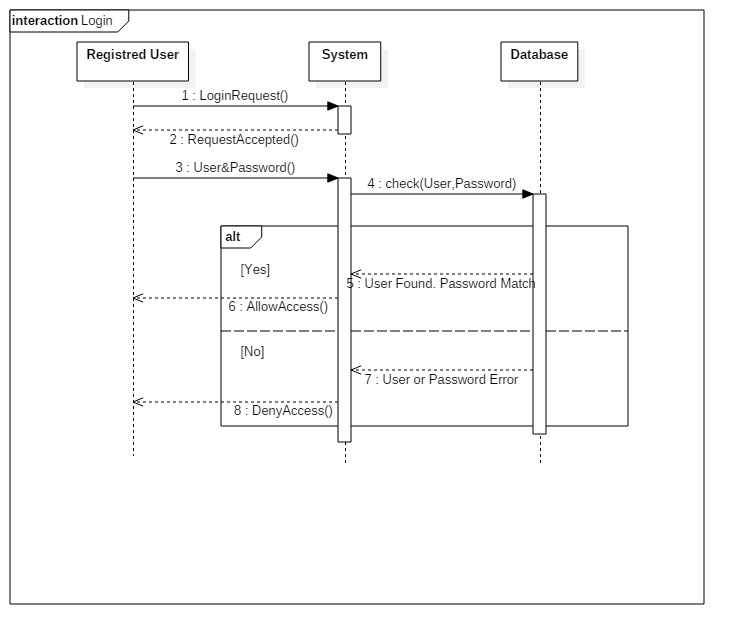
\includegraphics[width=6in]{./diagrams/SequenceLogin.png}
	\caption{Sequence Diagram: Login}
	\label{fig:SequenceLogin}
\end{figure}

\subsection*{Create Meeting}
\begin{center}

	\begin{tabular}{|c||p{0.6\textwidth}|}
		\hline
		Name & Create appointment \\ \hline
		Actors & User \\ \hline
		Assumption & The user need to insert a new appointment in his personal calendar \\ \hline
		Pre-Conditions & \begin{itemize}
			\item The user has successfully signed to the system
			\item The user has already opened the window with the insertion form.
		\end{itemize} \\ \hline
		Flow of events & \begin{enumerate}
			\item The user creates a new appointment by inserting all the information needed in order to adding a new event correctly in his own calendar.
			\item The system check into the calendar if the location of the appointment is reachable in the allotted time or if the event is overlapping with other appointment.
			\item The user is informed by a warning message about the actual validation of the appointment.
			\item The user have to confirm o reject the insertion of the appointment
		\end{enumerate} \\ \hline
		Post-Conditions & The appointment of the user has been stored to the system in the event that he has confirmed the inclusion. \\ \hline
		Exception & An internal system error makes impossible to store the reservation data. The user is notified of the error \\ \hline		
	\end{tabular}
\end{center}

\begin{figure}[H]
	\centering
	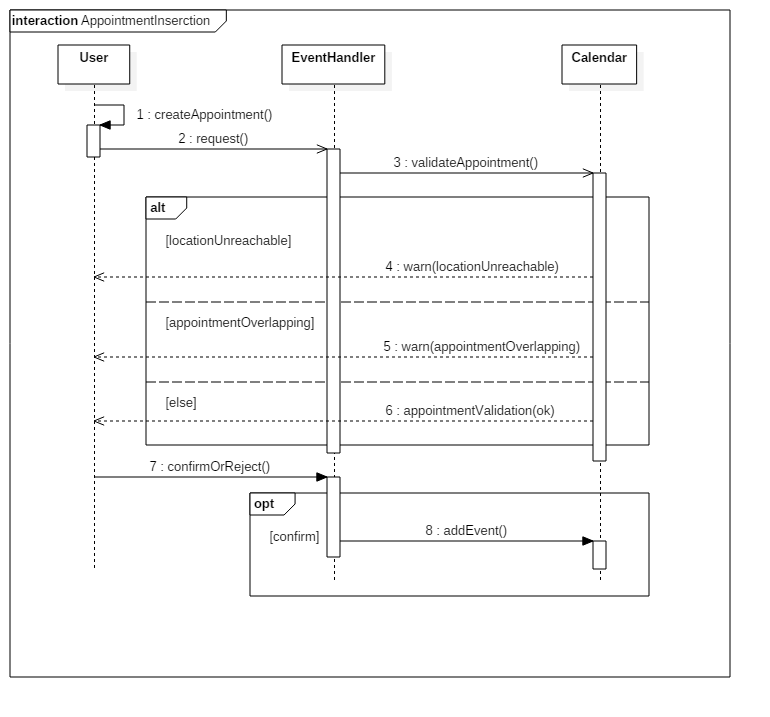
\includegraphics[width=6in]{./diagrams/AppointmentInserction.png}
	\caption{Sequence Diagram: Create Appointment}
	\label{fig:SequenceAddApp}
\end{figure}

[TODO] Mockups to be transferred when the use will be finished.

\begin{figure}[H]
	\caption{Main application landing}
	\centerline{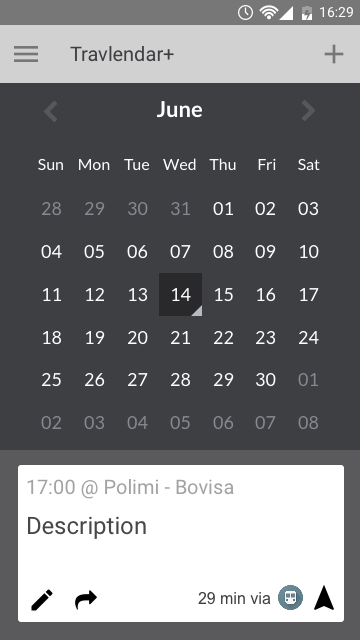
\psfig{file=images/home.png,width=0.6\textwidth} } 
\end{figure}
\begin{figure}[H]
	\caption{Menu view}
	\centerline{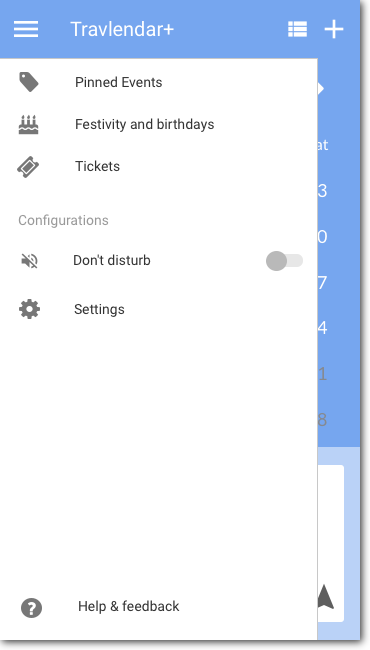
\psfig{file=images/menu.png,width=0.6\textwidth} }
\end{figure}
\begin{figure}[H]
	\caption{Create a new appointment}
	\centerline{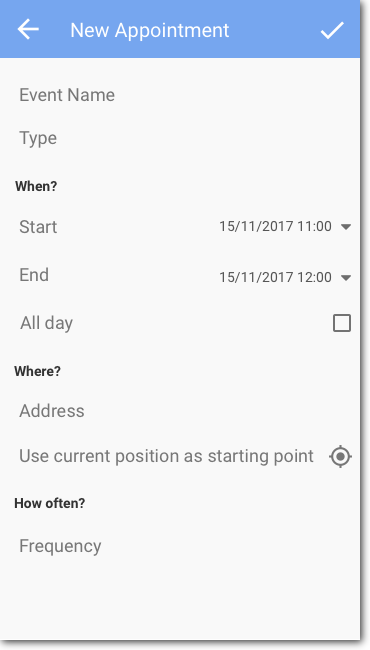
\psfig{file=images/appointment.png,width=0.6\textwidth} }
\end{figure}
\begin{figure}[H]
	\caption{Listing view of the appointments}
	\centerline{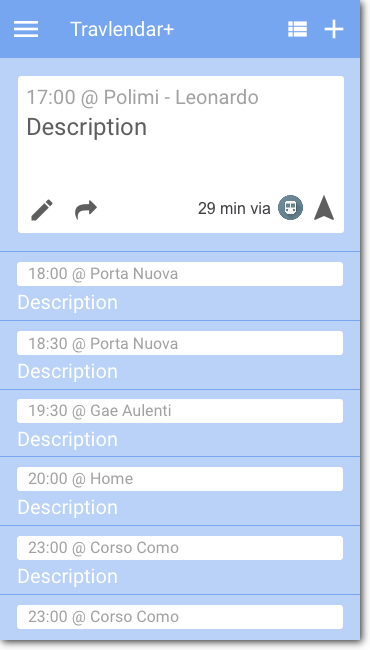
\psfig{file=images/listing.png,width=0.6\textwidth} }
\end{figure}
\begin{figure}[H]
	\caption{Notification from the application}
	\centerline{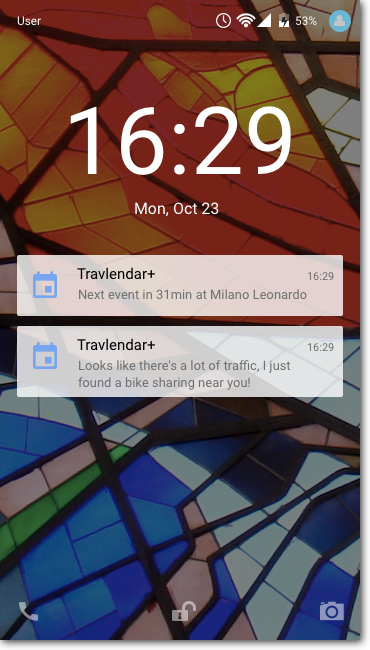
\psfig{file=images/lockscreen.png,width=0.6\textwidth} }
\end{figure}
\begin{figure}[H]
	\caption{Login}
	\centerline{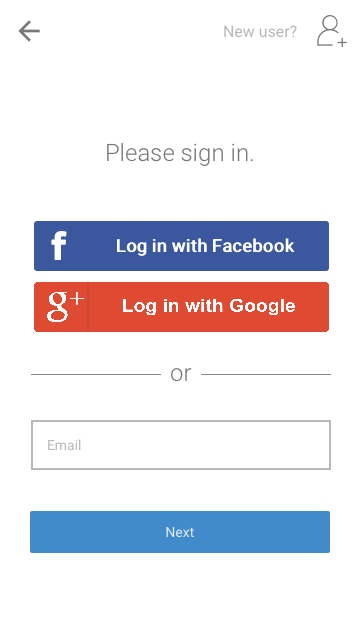
\psfig{file=images/login.png,width=0.6\textwidth} }
\end{figure}
\begin{figure}[H]
	\caption{Navigation with car}
	\centerline{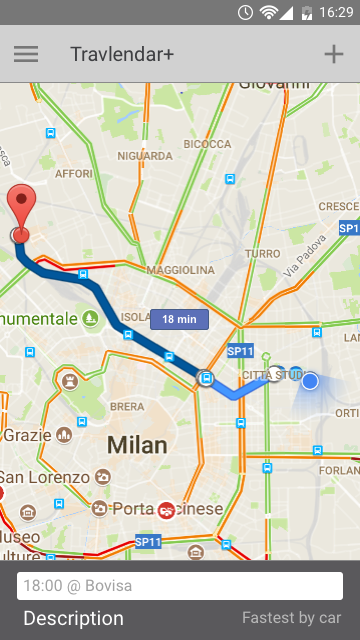
\psfig{file=images/map_car.png,width=0.6\textwidth} }
\end{figure}
\begin{figure}[H]
	\caption{Navigation with public transport}
	\centerline{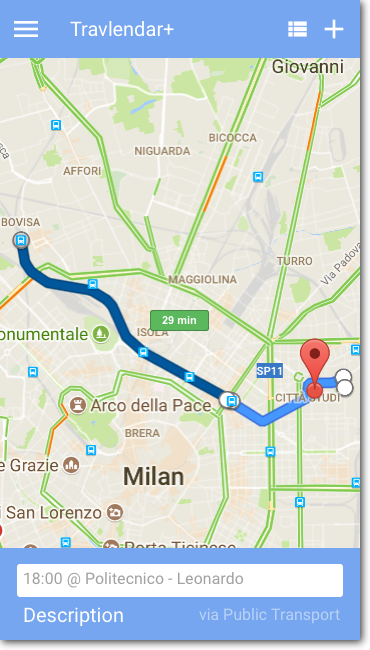
\psfig{file=images/map_pt.png,width=0.6\textwidth} }
\end{figure}
\begin{figure}[H]
	\caption{Settings}
	\centerline{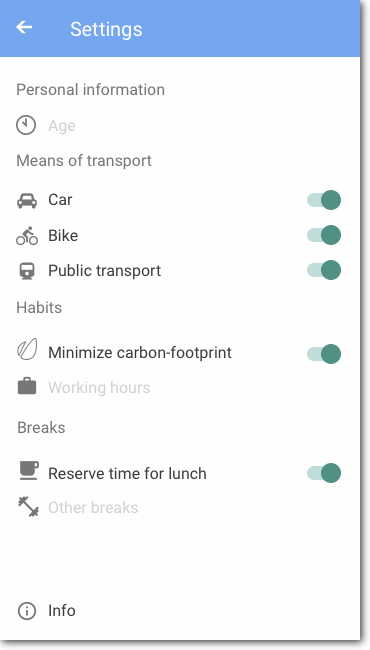
\psfig{file=images/settings.png,width=0.6\textwidth} }
\end{figure}

\section{Performance Requirements}
\label{sec:perf_req}
The user experience across the application should be fluid and with zero waiting time moving between the sections. Besides, there are a number of requirements that implies third party information retrieved through asynchronous requests so, the previous requirement can allow some tolerance.

\begin{enumerate}
\item There is no limit to the number of users registered to the application.
\item There is no limit to the number of the simultaneous users of the application.
\item The login process must be completed in less than 5 seconds once submitted the data.
\item The date text fields have to validate dates in real time.
\item The application going back to foreground has to be in the same state as when it was going to background
\end{enumerate}


\section{Design Constraints}
\label{sec:design_constraints}

\subsection{Standards compliance}
The application will be developed with the MVVM architectural pattern to allow the unification of the business logic and the coherence across all the various implementations.
The implementation on iOS and Android will be compliant with the App Store Review guidelines and Android Compatibility Definition Document.

\subsection{Hardware limitations}
The application relies on the usage of the GPS location and Internet access. In any case of disabled GPS or energy-saver option that blocks the retrieval of the User’s location or in case of no connectivity the application will not provide the user the ETA or the route navigation to reach an event nor the login function if the user is logged out.
\subsection{Any other constraint}
\input{requirements/other.tex}

\section{Software System Attributes}
\label{sec:sys_attribs}

\subsection{Reliability}
The application should have a 100 \% uptime in every designed scenario. Since the application relies on other systems API’s there will be the possibility to accept small variations in this requirement.
\subsection{Availability}
Regarding the mobile implementations the application will be available in the App Store and Play Store, instead, the desktop implementation will be available through the web app.
\subsection{Security}
The applications will perform every request in HTTPS to preserve the security of the user. 
Data that have to be stored in the device, will be encrypted with third-party libraries to avoid leakage of the user’s information.

\subsection{Maintainability}
The implementations will be developed with the MVVM architectural pattern allowing a modular integration of future new features or changes in the requirements. 
The application will rely on Google Maps API in order to maintain its core functionalities and not on other third-party libraries that could be deprecated in future OS versions.

\subsection{Portability}

\input{requirements/portability.tex}

		\newpage
		\chapter{Alloy Analysis}
\label{cha:alloy}

The following is a possible solution of the Alloy model. We present a completed version of such model in Figure \ref{fig:completeAlloy} and a reduced version with only the main entities, shown in Figure \ref{fig:reducedAlloy}.
\lstinputlisting[language=alloy]{./alloy/alloy_model.als}

\begin{sidewaysfigure}
    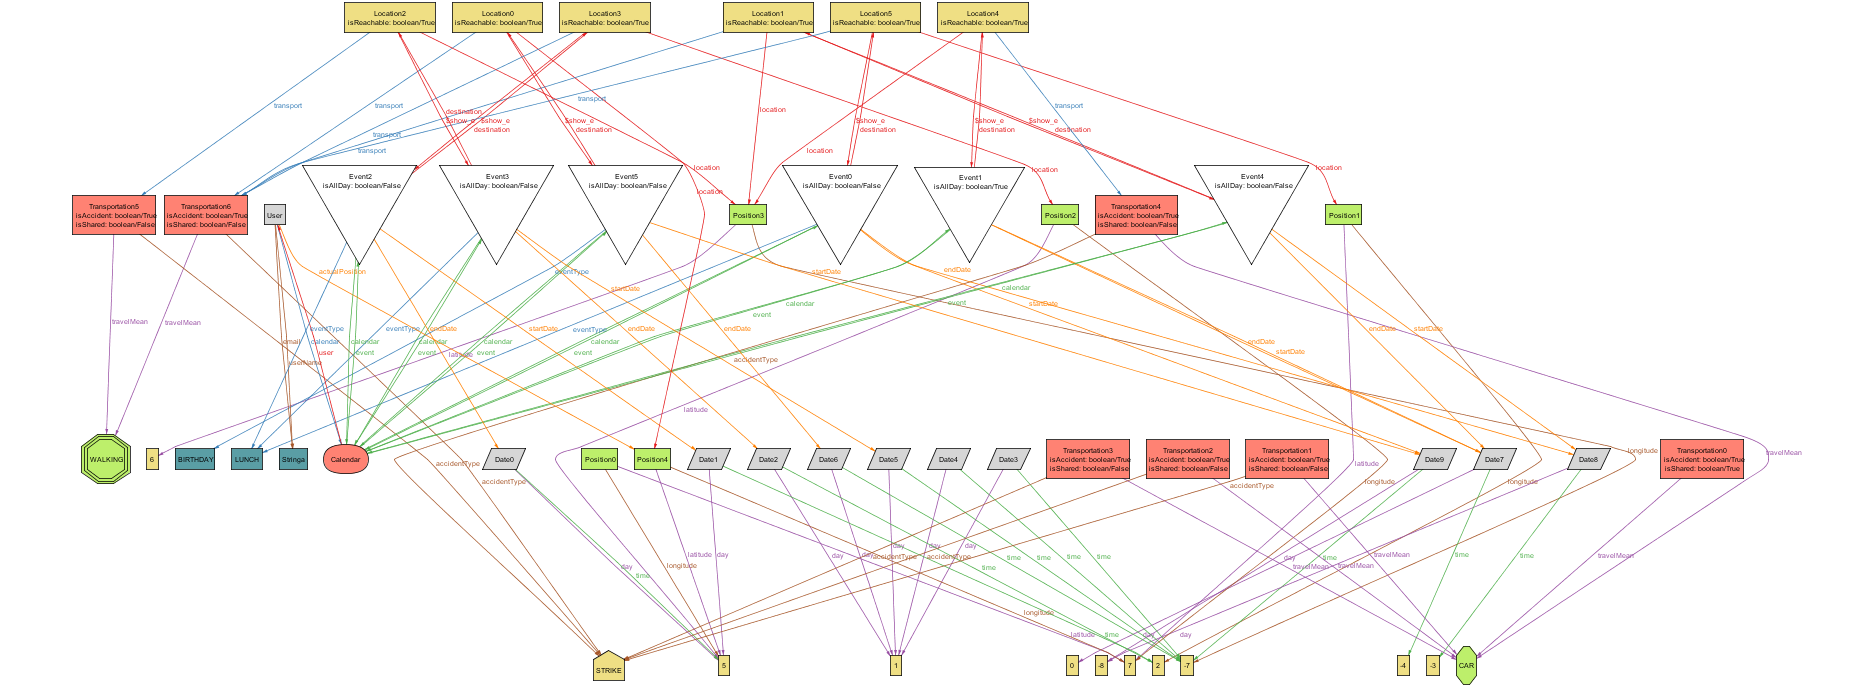
\includegraphics[width=\textwidth]{./alloy/complete_version.png}
    \caption{Alloy model (complete version).}
    \label{fig:completeAlloy}
\end{sidewaysfigure}

\begin{sidewaysfigure}
    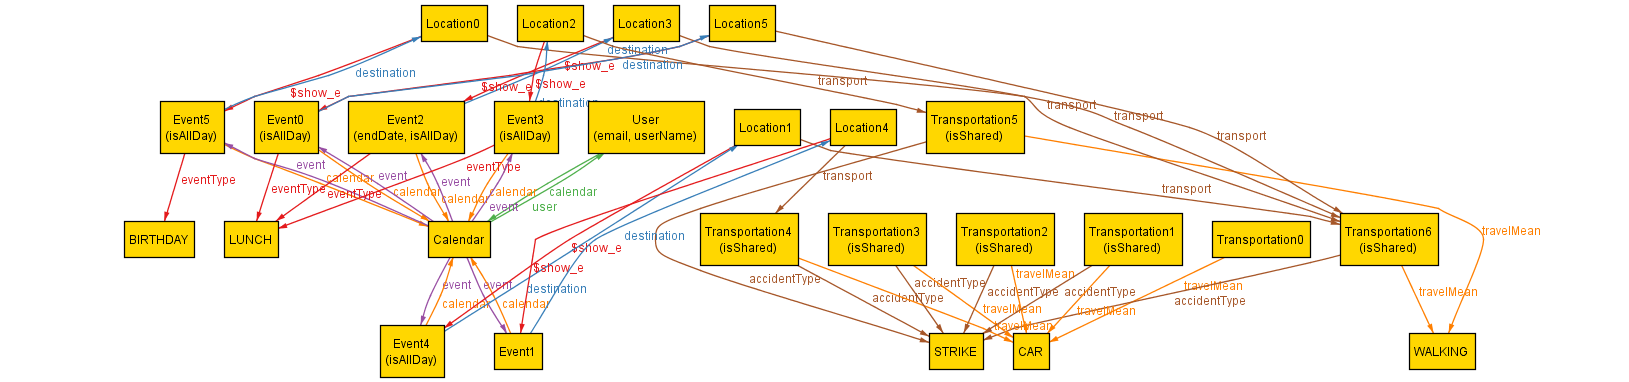
\includegraphics[width=\textwidth]{./alloy/reduced_version.png}
    \caption{Alloy model (reduced version).}
    \label{fig:reducedAlloy}
\end{sidewaysfigure}

	\endgroup
    
    \addcontentsline{toc}{chapter}{Bibliography}
    \bibliographystyle{unsrt}
    \bibliography{biblio}

	\appendix
	\chapter*{Appendix}
\addcontentsline{toc}{chapter}{Appendix}
\end{document}
